\documentclass[conference]{IEEEtran}
\IEEEoverridecommandlockouts
% The preceding line is only needed to identify funding in the first footnote. If that is unneeded, please comment it out.
\usepackage{cite}
\usepackage{amsmath,amssymb,amsfonts}
\usepackage{algorithmic}
\usepackage{graphicx}
\usepackage{textcomp}
\usepackage{xcolor}
\usepackage{booktabs} 
\usepackage{makecell} 
\usepackage{multirow} 
\usepackage{siunitx} 
\usepackage{pifont}
\newcommand{\cmark}{\ding{51}}%
\newcommand{\xmark}{\ding{55}}%
\usepackage{tikz}
\usetikzlibrary{patterns.meta,backgrounds, calc, arrows.meta, intersections, patterns, positioning, shapes.misc, fadings, through,decorations.pathreplacing,shapes}
\usepackage{caption}
\usepackage{enumitem}
\usepackage{listofitems}
\usepackage{changepage}
\usepackage{listings}

% Enable or disable reviews
\newif\ifreview
\reviewtrue
%\reviewfalse

\definecolor{amber}{rgb}{1.0, 0.75, 0.0}
\newcounter{ReviewerID}
\readlist*\annotationcolors{blue, red, orange, green, purple, amber, brown, olive}
\newcommand{\newreviewer}[2]{%
        \ifnum \theReviewerID=\annotationcolorslen
        \setcounter{ReviewerID}{0} % cycle through colors
        \fi
        \stepcounter{ReviewerID}%
        \expandafter\edef\csname bootstrap#1\endcsname{%
                \expandafter\def\csname #1\endcsname####1{%
                        \ifreview%
                         {\noexpand\color{\annotationcolors[\theReviewerID]} {\noexpand\bf{\noexpand\fbox{#2}} {\noexpand\it ####1} }}
                        \else%
                         {}% disable annotations
                        \fi%
                }%
        }%
        \csname bootstrap#1\endcsname%
}



\makeatletter
\let\old@lstKV@SwitchCases\lstKV@SwitchCases
\def\lstKV@SwitchCases#1#2#3{}
\makeatother
\usepackage{lstlinebgrd}
\makeatletter
\let\lstKV@SwitchCases\old@lstKV@SwitchCases

\lst@Key{numbers}{none}{%
    \def\lst@PlaceNumber{\lst@linebgrd}%
    \lstKV@SwitchCases{#1}%
    {none:\\%
     left:\def\lst@PlaceNumber{\llap{\normalfont
                \lst@numberstyle{\thelstnumber}\kern\lst@numbersep}\lst@linebgrd}\\%
     right:\def\lst@PlaceNumber{\rlap{\normalfont
                \kern\linewidth \kern\lst@numbersep
                \lst@numberstyle{\thelstnumber}}\lst@linebgrd}%
    }{\PackageError{Listings}{Numbers #1 unknown}\@ehc}}
\makeatother



\newreviewer{yiwen}{yiwen}
\newreviewer{mat}{mat}

\def\BibTeX{{\rm B\kern-.05em{\sc i\kern-.025em b}\kern-.08em
    T\kern-.1667em\lower.7ex\hbox{E}\kern-.125emX}}
\begin{document}

\title{Evolution of Rust for Linux: From Unsafe to Safe}

\author{\IEEEauthorblockN{Yiwen Xu}
\IEEEauthorblockA{
\textit{École Polytechnique Fédérale de Lausanne (EPFL)}\\
Lausanne, Switzerland}
% \and
% \IEEEauthorblockN{6\textsuperscript{th} Given Name Surname}
% \IEEEauthorblockA{\textit{dept. name of organization (of Aff.)} \\
% \textit{name of organization (of Aff.)}\\
% City, Country \\
% email address or ORCID}
}

\maketitle

\begin{abstract}
Linux has been the de facto operating system for servers and desktop computers for decades, yet it has been plagued by a number of security vulnerabilities.
A significant cause is that, for performance reasons, the kernel is written in C, a language that is not memory-safe by design. For this reason, the Linux kernel community has been exploring the use of memory-safe languages to improve the security of the kernel.
Rust, as a modern system programming language with security at its core, has gained popularity in the Linux kernel community. Therefore, the Rust for Linux project was initiated to add the fundamental support for Rust development to the Linux kernel, following by many practices on new or old drivers being rewritten in Rust.

Driver development cannot exist independently of the existing kernel subsystems, which poses a significant challenge for the Rust for Linux project: how can idiomatic Rust be integrated elegantly into the existing kernel without disrupting its infrastructure, while still coexisting seamlessly with the remaining C code? 


To help shape the ongoing works of Rust drivers and other Rust--C
systems-level projects, we present a comprehensive study of the evolution
of Rust for Linux, from the initial introduction of Rust support to the
current state-of-the-art design and the disciplined use of \texttt{unsafe}
blocks. 
First, we examine the design choices behind the abstraction layers
that bridge Rust and C. 
Second, we analyze the rationale for \texttt{unsafe}
Rust usage---the only source of residual memory-safety issues---and
trace its evolution across different abstraction layers and drivers in the kernel.
Finally, we distill the practical guidelines and best practices
that have emerged from the Rust for Linux project for future development.

This study is both timely and necessary, as Rust has moved from an
experimental effort to an increasingly established part of kernel development.
Its growing adoption has also intensified interest in rewriting kernel
components and other systems-level software in Rust, especially where existing
C implementations have suffered from recurring memory-safety issues.


\end{abstract}

\begin{IEEEkeywords}
Trusted Execution Environment, Bug Detection, Double Fetch Vulnerabilities
\end{IEEEkeywords}

\section{Introduction}



The Linux kernel has underpinned modern computing infrastructure for over three decades, running on everything from embedded devices and smartphones
to cloud servers and supercomputers. Yet, despite its maturity and widespread deployment, the kernel remains a persistent source of critical security
vulnerabilities. Memory safety errors---buffer overflows, use-after-free, null-pointer dereferences, and out-of-bounds accesses---account for a disproportionate fraction of reported kernel CVEs. 

Empirical analyses of the Linux CVE database consistently show that a majority of high-severity vulnerabilities trace back to memory unsafety~\cite{TODO:cve_study,TODO:linux_memory_bugs}, a fundamental consequence of the kernel being written in C, a language that offers no compile-time guarantees over memory accesses and relies entirely on programmer discipline for correctness. Furthermore, in the LLM era, the number of vulnerabilities reported by LLMs to Linux kernel has increased significantly, making it more difficult to Linux community to patch vulnerabilities in a timely manner~\cite{TODO:llm_vulnerabilities_to_linux}.

Rust~\cite{TODO:rust_book} has emerged as a feasible and principled response to this challenge. As a modern system programming language with memory safety and efficiency as its core design goals, Rust enforces strict ownership, borrowing, and lifetime rules through its type system and borrow checker, statically and dramatically eliminating most classes of memory errors at compile time. Unlike garbage-collected languages, it is crucial to note that Rust achieves these guarantees without a runtime overhead, preserving the low-level control and performance required for kernel development.

Motivated by these properties, the Rust for Linux project~\cite{TODO:ojeda2022rust, TODO:rustforlinux} was initiated to introduce Rust as a second implementation language in the Linux kernel. The goal is not to rewrite the existing kernel in Rust, but to allow newly-involved security-critical drivers and kernel subsystems to be developed in idiomatic, safe Rust.
After extensive preparatory work spanning several years, Rust support was merged into the mainline kernel at Linux~v6.1~\cite{TODO:linux_v6.1}. Today, Rust is widely regarded as a successful second language in the kernel community, and its status has continued to mature following the removal of the ``experimental'' label in Linux~v6.19~\cite{TODO:linux_v6.19}.
The project follows a layered architecture: the existing C kernel infrastructure forms the foundation; a thin layer of \texttt{unsafe} Rust bindings bridges Rust to the C~APIs; an elaborately-designed and carefully-reviewed \emph{safe abstraction layer} wraps these bindings and exposes ergonomic, safe Rust interfaces; and Rust drivers are then built on top of this abstraction layer.
This design localizes majority of \texttt{unsafe} blocks, the only source of memory safety issues in Rust code, to the abstraction layer and shields the leaf driver code from direct C interoperability hazards and the associated security risks.

Despite this architecture, Rust's memory safety guarantees are not absolute in the kernel context. 
The \texttt{unsafe} keyword marks code regions where the compiler relaxes its safety invariants, permitting raw pointer
dereferences, foreign function calls to C, and other low-level operations.
In Rust for Linux, \texttt{unsafe} blocks are an unavoidable necessity:
the fundamental mismatch between Rust's strict ownership model and C's type
system---in particular around pointer aliasing, validity, and lifetime
management---means that no safe abstraction can be built without an
\texttt{unsafe} foundation.
The project therefore adopts a discipline: \texttt{unsafe} code should be
confined to the abstraction layers, rigorously documented, and individually
justified, so that driver code above can remain \texttt{unsafe}-free.
Our study reveals that \texttt{unsafe} usage is not uniformly distributed
across the kernel's Rust codebase; it is heavily concentrated in the
abstraction layer, while driver-level code remains largely free of explicit
\texttt{unsafe} blocks (see Figure~\ref{fig:unsafe_dist} and
Table~\ref{tab:unsafe_stats}). % TODO: fill in figure and table

Prior research has examined Rust security from two complementary angles.
A first line of work focuses on automated detection of \texttt{unsafe} bugs
in the broader Rust ecosystem.
RUDRA~\cite{TODO:bae2021rudra} performs inter-procedural dataflow analysis
to find unsound patterns in unsafe Rust APIs, targeting violations of
higher-order safety invariants and incorrect \texttt{Send}/\texttt{Sync}
implementations commonly found in published crates.
SafeDrop~\cite{TODO:safedrop} targets use-after-free and double-free
vulnerabilities by tracking ownership transfer and drop semantics through a
path-sensitive analysis of Rust's Mid-level Intermediate Representation
(MIR), making it effective at catching lifetime-related misuse.
TypePulse~\cite{TODO:typepulse} takes a type-confusion-centric approach,
identifying bugs that arise from unsound type casts in \texttt{unsafe}
code---a vulnerability class of particular relevance at FFI boundaries
where Rust and C types are coerced into one another.
While all three tools target \texttt{unsafe}-related memory bugs, they
differ in their underlying representations, targeted vulnerability classes,
and scope: RUDRA and SafeDrop are designed for the Rust crate ecosystem,
whereas TypePulse is specifically oriented toward cross-language type safety
at FFI boundaries.

A second, complementary line of work takes an empirical perspective on
Rust's integration into the Linux kernel itself.
Li et al.~\cite{TODO:li2024empirical} conducted the first large-scale
qualitative study of the Rust for Linux project through developer mailing
lists, patch discussions, and issue reports, documenting sources of success,
dissatisfaction, and compromise in the project's early stages.
While this study provides valuable sociological and high-level architectural
insight, it is necessarily broad: it was conducted before the project had
reached sufficient maturity to include complex, production-quality driver
examples, and it does not systematically analyze the design and safety
properties of the abstraction layer, nor does it characterize how
\texttt{unsafe} is justified and distributed within it.

In this paper, we present the first systematic study of the evolution of
Rust for Linux, with a focus on the design and safety of its abstraction
layers and the disciplined use of \texttt{unsafe} Rust in real kernel code.
We trace how the Rust-C interface has been designed and refined over
successive kernel releases, systematically analyze the rationale behind
\texttt{unsafe} usage across the full abstraction stack, and distill the
practical guidelines and best practices that have emerged from the project
for future Rust kernel development.

\medskip
\noindent\textbf{Contributions.} This paper makes the following contributions:

\begin{itemize}[leftmargin=*]
    \item \textbf{Architectural analysis.} We provide a comprehensive
    longitudinal analysis of the Rust for Linux abstraction layer design,
    tracing its evolution from the initial Rust support in Linux~v6.1 to the
    current state of the art, and characterizing the key design decisions that
    govern Rust-C interoperability.

    \item \textbf{Unsafe characterization.} We systematically study the
    distribution, rationale, and evolution of \texttt{unsafe} blocks across
    abstraction layers and drivers in the Rust for Linux codebase, revealing
    consistent patterns in how and why \texttt{unsafe} is used and how these
    patterns have changed as the project has matured.

    \item \textbf{Design guidelines.} We distill a set of practical design
    principles and best practices for writing safe Rust kernel code, grounded
    in the hard-won experience of the Rust for Linux project and intended to
    guide future development of Rust-based kernel components and other
    Rust-C systems-level software.
\end{itemize}



\section{Background}
\label{sec:bak}
{\bf TEE on Android}.
To mitigate the security risks inherent in monolithic kernels, the mobile industry has adopted the TEE to guarantee code integrity and data confidentiality~\cite{bove2024large, sabt2015trusted}. On Android devices, this is predominantly implemented via ARM TrustZone technology~\cite{pinto2019demystifying}, which partitions the processor into two distinct execution states: the normal world for the rich operating system and the secure world for the Trusted OS. This hardware-backed isolation ensures that sensitive resources remain protected even if the Android kernel is compromised. Transitions between these worlds are mediated by Secure Monitor, typically triggered by Secure Monitor Calls (SMC)~\cite{ngabonziza2016trustzone}. Within the secure world, vendor-specific Trusted Operating Systems—such as Qualcomm’s QSEE, Samsung’s TEEGris, or Xiaomi’s MiTEE—manage Trusted Applications (TAs), which are signed binaries executing specific security-critical logic~\cite{9152801}.

{\bf Communication Mechanism}.
The utility of the TEE relies on the GlobalPlatform TEE Client API specification, which standardizes the communication interface between Client Applications (CAs) in the normal world and TAs in the secure world~\cite{teeAPI, suzaki2020library}. To facilitate high-throughput operations, such as high-definition DRM content processing or biometric authentication, the specification supports Shared Memory mechanisms. This allows the TEE to access data structures located in the normal world's memory without the performance overhead of copying large buffers into the restricted secure world memory. Specifically, the API utilizes operations like \texttt{TEEC\_InvokeCommand} to pass parameters, which often include references to memory buffers (\texttt{TEEC\_MEMREF}) that act as the conduit for zero-copy data exchange.

In practice, vendors prioritize these zero-copy transfer methods to maximize system performance, mapping the physical pages of the Client Application's buffer directly into the virtual address space of the Trusted Application. While efficient, this shared access model creates a scenario where the secure execution operates on data residing in unsecure physical RAM~\cite{machiry2017boomerang}. Consequently, unless specific shadow buffer copying mechanisms are enforced, the normal world retains write access to these memory pages concurrently while the Trusted Application is reading from them. This shared visibility, lacking intrinsic hardware locking for concurrent access, establishes the architectural precondition for race conditions.

\begin{figure}[ht]
        \definecolor{pgreen}{rgb}{0,0.5,0}
\definecolor{pblue}{rgb}{0.13,0.13,1}
\definecolor{pred}{rgb}{0.9,0,0}
\definecolor{pgrey}{rgb}{0.46,0.45,0.48}
\definecolor{light-gray}{gray}{0.975}
\definecolor{darkgreen}{rgb}{0,0.5,0}
\definecolor{vscodepurple}{RGB}{128, 0, 128}
\definecolor{codepurple}{rgb}{0.58,0,0.82}

\lstset{escapechar=@,
                backgroundcolor = \color{light-gray},
                linebackgroundcolor={%
                \ifnum\value{lstnumber}>0
                    \ifnum\value{lstnumber}<30
                        \color{light-gray}
                    \fi
                \fi
                %\ifnum\value{lstnumber}>10
                %    \ifnum\value{lstnumber}<12
                %        \color{teal!40}
                %    \fi
                %\fi
                \ifnum\value{lstnumber}>15
                    \ifnum\value{lstnumber}<17
                        \color{blue!20}
                    \fi
                \fi 
                \ifnum\value{lstnumber}>20
                    \ifnum\value{lstnumber}<22
                        \color{red!20}
                    \fi
                \fi
                \ifnum\value{lstnumber}>22
                    \ifnum\value{lstnumber}<24
                        \color{red!20}
                    \fi
                \fi
                \ifnum\value{lstnumber}>23
                    \ifnum\value{lstnumber}<25
                        \color{red!20}
                    \fi
                \fi
                },
                tabsize=2,
                basicstyle=\fontencoding{T1}\selectfont\footnotesize,
                %basicstyle=\fontfamily{lmvtt}\selectfont\footnotesize,
                commentstyle=\color{darkgreen!80},
                keywordstyle=\color{pblue},
                stringstyle=\color{pred},
                %stringstyle=\color{vscodepurple},
                frame = single,
                showstringspaces=false,
                language=c,
                xleftmargin=5pt, 
                xrightmargin=5pt, 
                %framexleftmargin=-5pt,
                numbers=left,                  % Line numbers
                numberstyle=\tiny\color{black}, % Line number style
                numbersep=4pt, %moredelim=[is][\textbf]{@}{@}
                %escapeinside={(*@}{@*)}
}
\center

\begin{lstlisting}[columns=fullflexible]
typedef struct in_data{
    size_t size;
    char data[0];
} in_data;

int* global = NULL;

TEE_Result TA_InvokeCommandEntryPoint(
  int commandID, int param_types, TEE_Param params[4])
{
  if (param_types != 0x7) return -1;

  in_data* in = (in_data*)params[0].memref.buffer;
  size_t in_buf_sz = params[0].memref.size;
 
  size_t in_size = in->size; 
  if(in_size > in_buf_sz || in_size > 0x2000) return 0;

  char* copy_buf = TEE_Malloc(in_size, 0);
  if(commandID == 1){
    printf("[debug] called with size %zu\n", in->size);
  } else if (commandID == 2){
    memcpy(copy_buf, in->data, in->size);
  } else if (commandID == 3 && in->size == 1234){
    *global = 1;
   }
  return 0;
}
\end{lstlisting}

        \captionof{lstlisting}{
            \yiwen{double check references and line numbers}
           A TA's \texttt{TA\_InvokeCommandEntryPoint} function. The TA expects a single
           argument buffer, containing an \texttt{in\_data} structure. The TA operates directly on the shared memory 
            (\texttt{params[0].memref.buffer}) and ends up having three double fetches.
           The first fetch is marked in \colorbox{blue!40}{blue} and the second fetches are marked in \colorbox{red!40}{red}.
           While the double fetch on line 21 is harmless, the double fetch on line 23 may lead to a heap buffer overflow if 
           a malicious NWCA modifies the value of \texttt{in->size} between lines 16 and 23. The code path of the double 
           fetch on line 24 leads to a null pointer dereference, however this bug is triggerable without shared memory 
            double fetches.
        }
        \label{lst:exdf}
\end{figure}

\textbf{Double Fetch Vulnerabilities}.
While the shared memory mechanism is essential for performance, it introduces a critical attack surface where the untrusted normal world can modify data concurrently while the secure world processes it. This lack of hardware-enforced synchronization gives rise to Double Fetch vulnerabilities, a specific form of Time-of-Check to Time-of-Use (TOCTOU) race condition inherent to TEEs~\cite{wang2017double, schwarz2018automated}. A Double Fetch occurs when a privileged Trusted Application reads a value from the shared buffer twice: first to validate constraints (such as a buffer size check) and second to actually use the value (such as in a memory copy). An attacker controlling the normal world can exploit the race window between these two accesses to modify the memory content, changing a safe value to a malicious one after validation. This effectively bypasses the security check, leading to critical failures like heap overflows or arbitrary code execution within the secure perimeter~\cite{xu2018precise}.

These vulnerable double fetches are of particular interest to attackers as they provide a direct path to compromise the TEE. By exploiting these flaws from the normal world, an adversary can achieve code execution within the vulnerable TA, effectively allowing them to pivot from the untrusted OS into the secure world. Furthermore, the issue is exacerbated by the design of TEE development environments compared to other privileged contexts. Unlike the Linux kernel, where access to untrusted memory is made explicit through mechanisms like \texttt{copy\_from\_user}, the TEE context typically exposes shared memory via raw pointers without such safeguards. Consequently, there is no enforced mechanism to ensure atomicity, placing the entire burden of securely handling \texttt{memref} buffer pointers and preventing race conditions solely on the TA developer.




\section{Design}


\begin{figure*}[h!]
    \centering
    \begin{figure*}[t]
    \centering
    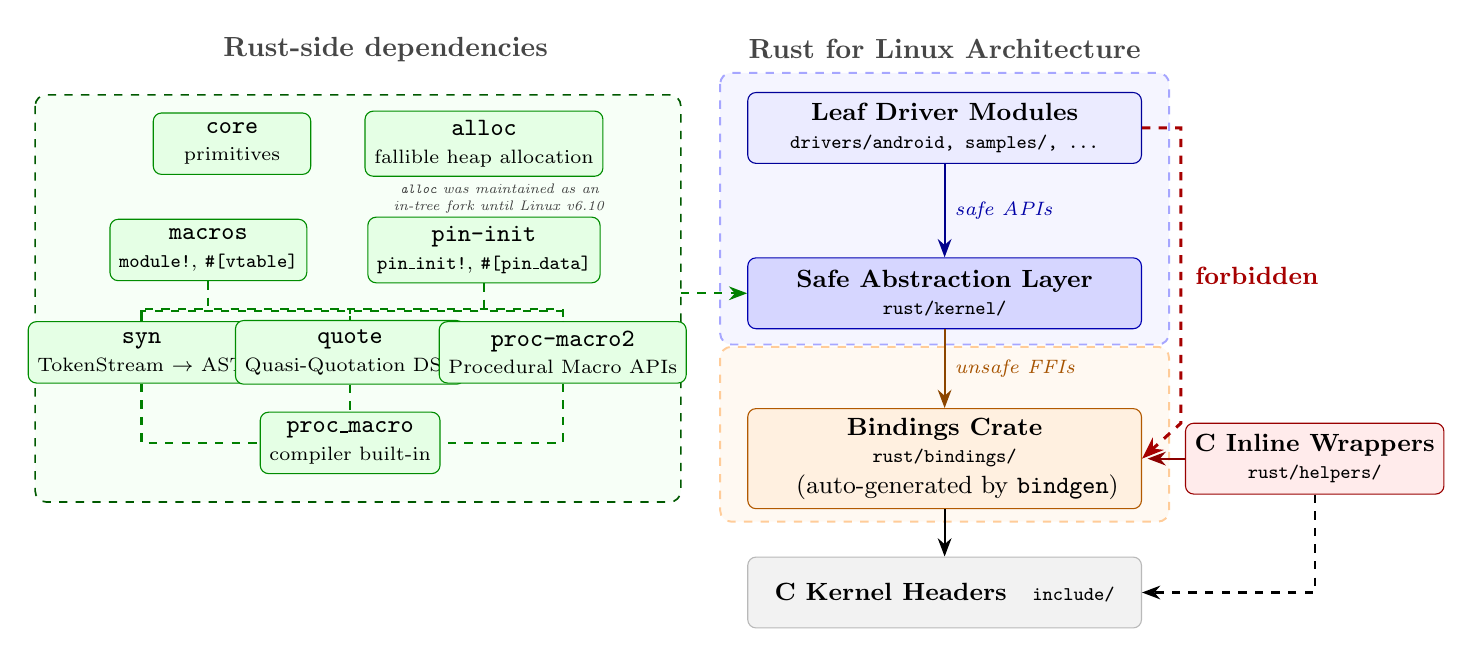
\begin{tikzpicture}[
        xshift=0.45cm,
      %% Node styles
      safenode/.style  = {draw=blue!60!black,  fill=blue!8,    rounded corners=3pt,
                          minimum width=5.0cm, minimum height=0.90cm,
                          align=center, font=\small},
      corenode/.style  = {draw=blue!70!black,  fill=blue!16,   rounded corners=3pt,
                          minimum width=5.0cm, minimum height=0.90cm,
                          align=center, font=\small},
      unsafenode/.style= {draw=orange!70!black,fill=orange!12, rounded corners=3pt,
                          minimum width=5.0cm, minimum height=0.90cm,
                          align=center, font=\small},
      cheadnode/.style = {draw=gray!55,        fill=gray!10,   rounded corners=3pt,
                          minimum width=5.0cm, minimum height=0.90cm,
                          align=center, font=\small},
      upnode/.style    = {draw=green!55!black, fill=green!10,  rounded corners=3pt,
                          minimum width=2.0cm, minimum height=0.78cm,
                          align=center, font=\small},
      sidenode/.style  = {draw=red!60!black,  fill=red!8,    rounded corners=3pt,
                            minimum width=3.0cm, minimum height=0.90cm,
                            align=center, font=\small},
      %% Arrow styles
      main/.style    = {-Stealth, thick},
      safefl/.style  = {-Stealth, thick, blue!55!black},
      unsafefl/.style= {-Stealth, thick, orange!55!black},
      sidenefl/.style= {-Stealth, thick, red!55!black},
      %% green legs: no arrowhead; trunk has arrowhead
      leg/.style     = {thick, green!50!black, dashed},
      depfl/.style   = {-Stealth, thick, green!50!black, dashed},
      forbid/.style  = {-Stealth, line width=1.1pt, red!65!black, dashed},
    ]
    
    %% ── Main vertical stack (centre, box half-width = 2.5 cm) ────────────
    \node[safenode]   (drivers)  at (0.8,  0.0)
      {\textbf{Leaf Driver Modules}\\[-1pt]
       {\scriptsize\texttt{drivers/android, samples/, ...}}};
    
    \node[corenode]   (kernel)   at (0.8, -2.1)
      {\textbf{Safe Abstraction Layer}\\[-1pt]
       {\scriptsize\texttt{rust/kernel/}}};
    
    \node[unsafenode]  (bindings) at (0.8, -4.2)
      {\textbf{Bindings Crate}\\[-1pt]
       {\scriptsize\texttt{rust/bindings/}} \\ \quad(auto-generated by \texttt{bindgen})};
    
    \node[cheadnode]  (include)  at (0.8, -5.9)
      {\textbf{C Kernel Headers}\quad{\scriptsize\texttt{include/}}};
    
    %% ── Flow arrows (vertical) ───────────────────────────────────────────
    \draw[safefl]   (drivers.south)  --
      node[right, font=\scriptsize, blue!65!black]{\textit{safe APIs}}
      (kernel.north);
    \draw[unsafefl] (kernel.south)   --
      node[right, font=\scriptsize, orange!65!black]{\textit{unsafe FFIs}}
      (bindings.north);
    \draw[main]     (bindings.south) -- (include.north);
    
    %% ── helpers (right side of bindings) ─────────────────────────────────
    %  helpers.west = 4.5 cm;  bindings.east = 2.5 cm  →  clear gap

    \node[sidenode]  (helpers) at (5.5, -4.2)
      {\textbf{C Inline Wrappers}\\[-1pt]
       {\scriptsize\texttt{rust/helpers/}}};
    
    \draw[sidenefl, shorten >=2pt] (helpers.west) -- (bindings.east);
    %  helpers → include: go down then left
    \draw[main, dashed] (helpers.south) |- (include.east);
    
    %% ── FORBIDDEN arc ────────────────────────────────────────────────────
    %  Route: drivers.east → (3.8, 0) → (3.8, -3.75) → bindings.north east
    %  bindings.north is at y = -4.2 + 0.45 = -3.75
    %  Arc stays between boxes (right edge 2.5) and helpers (left edge 4.5)
    \coordinate (farc_top) at (3.8,  0.0);
    \coordinate (farc_bot) at (3.8, -3.75);
    
    \draw[forbid]
      (drivers.east) -- (farc_top)
                     -- (farc_bot)
                     -- (bindings.east);   %% = bindings.north east
    
    \node[font=\small\bfseries, red!65!black, right=0.06cm]
      at ($(farc_top)!0.5!(farc_bot)$) {forbidden};
    
    %% ── Upstream Rust (left) ─────────────────────────────────────────────
    %  upstream.east = -4.5 cm;  kernel.west = -2.5 cm
    %  Merge point at (-3.4, -2.1) keeps all routing strictly left of
    %  the safe-zone box border (-2.8 cm).
%% ── Rust-side dependencies (left) ────────────────────────────────────
\node[font=\bfseries, gray!55!black] at (-6.3, 1)
  {Rust-side dependencies};


  \node[font=\bfseries, gray!55!black] at (0.8, 1)
  {Rust for Linux Architecture};

%% Core / alloc remain independent
\node[upnode] (core) at (-8.25, -0.20)
  {\texttt{core}\\[-1pt]{\scriptsize primitives}};

\node[upnode] (allocu) at (-5.05, -0.20)
  {\texttt{alloc}\\[-1pt]{\scriptsize fallible heap allocation}};

\node[font=\tiny, gray!50!black, align=center, text width=3.2cm]
  at (-4.85, -0.90)
  {\textit{\texttt{alloc} was maintained as an in-tree fork until Linux~v6.10}};

\node[upnode, minimum width=2.25cm] (rflmacros) at (-8.55, -1.55)
  {\texttt{macros}\\[-1pt]
   {\scriptsize \texttt{module!}, \texttt{\#[vtable]}}};

\node[upnode, minimum width=2.25cm] (pininit) at (-5.05, -1.55)
  {\texttt{pin-init}\\[-1pt]
   {\scriptsize \texttt{pin\_init!}, \texttt{\#[pin\_data]}}};

\node[upnode, minimum width=1.25cm] (syn) at (-9.40, -2.85)
  {\texttt{syn}\\[-1pt]{\scriptsize TokenStream $\rightarrow$ AST}};

\node[upnode, minimum width=1.25cm] (quote) at (-6.75, -2.85)
  {\texttt{quote}\\[-1pt]{\scriptsize Quasi-Quotation DSL}};

\node[upnode, minimum width=1.65cm] (pm2) at (-4.05, -2.85)
  {\texttt{proc-macro2}\\[-1pt]{\scriptsize Procedural Macro APIs}};

\node[upnode, minimum width=2.15cm] (procmacro) at (-6.75, -4.00)
  {\texttt{proc\_macro}\\[-1pt]
   {\scriptsize compiler built-in}};

% left-side vertical bus and merge points
\coordinate (rust_bus_top) at (-3.25, -0.20);
\coordinate (rust_bus_mid) at (-3.25, -1.55);
\coordinate (rust_bus_in)  at (-2.80, -2.10);


%% macro infrastructure routing: use one lower bus
\coordinate (macro_bus) at (-6.05, -2.25);

\draw[leg] (rflmacros.south) -- ++(0,-0.35) -| (syn.north);
\draw[leg] (rflmacros.south) -- ++(0,-0.35) -| (quote.north);
\draw[leg] (rflmacros.south) -- ++(0,-0.35) -| (pm2.north);

\draw[leg] (pininit.south) -- ++(0,-0.35) -| (syn.north);
\draw[leg] (pininit.south) -- ++(0,-0.35) -| (quote.north);
\draw[leg] (pininit.south) -- ++(0,-0.35) -| (pm2.north);

% syn / quote / proc-macro2 to proc_macro, separated from main bus
\draw[leg] (syn.south)   |- (procmacro.west);
\draw[leg] (quote.south) -- (procmacro.north);
\draw[leg] (pm2.south)   |- (procmacro.east);
    
    %% ── Zone shading ─────────────────────────────────────────────────────
    \begin{scope}[on background layer]
        \fill[blue!4, rounded corners=4pt] (-2.05, 0.70) rectangle (3.65, -2.75);
        \draw[blue!35, rounded corners=4pt, dashed, line width=0.7pt]
                                          (-2.05, 0.70) rectangle (3.65, -2.75);
        
        \fill[orange!5, rounded corners=4pt] (-2.05,-2.78) rectangle (3.65, -5.0);
        \draw[orange!40, rounded corners=4pt, dashed, line width=0.7pt]
                                            (-2.05,-2.78) rectangle (3.65, -5.0);
    %   \node[font=\tiny, orange!60!black] at (2.50,-2.78) {unsafe};
    \end{scope}

    \begin{scope}[on background layer]
        \fill[green!3, rounded corners=4pt]
        (-10.75, 0.42) rectangle (-2.55, -4.75);
      \draw[green!35!black, dashed, rounded corners=4pt, line width=0.6pt]
        (-10.75, 0.42) rectangle (-2.55, -4.75);
    \end{scope}
    
    \draw[depfl]
    (-2.55, -2.10) -- (kernel.west);

    \end{tikzpicture}
    \caption{%
    Overview of the Rust for Linux architecture and its Rust-side dependencies.
    The left part depicts the Rust crates required by Rust for Linux, including upstream crates such as \texttt{core}
    and other supporting crates. In the middle part, leaf driver modules, such as
    \texttt{drivers/android} and \texttt{samples/}, are constrained to interact
    with the kernel through the safe abstraction layer in \texttt{rust/kernel/}, 
    which is built on top of the bindings and C helper wrappers to existing C kernel APIs.}
    \label{fig:rfl_arch}
    \end{figure*}
    \caption{
      Overview of SHMuzz. 
      }
    \label{fig:overview}
  \end{figure*}

  
Because shared memory is difficult to use safely and double-fetch bugs can result in severe memory corruption, We conduct the first dedicated study of double-fetch vulnerabilities in Trusted Applications. This effort requires an automated technique capable of uncovering attacker-triggerable flaws in large collections of proprietary, binary-only TAs.

To meet this need, We introduce SHMuzz, a dynamic, three-stage framework for detecting double-fetch vulnerabilities without access to source code. Although static analysis can theoretically examine all execution paths, it typically generates many false positives. In practice, most reported double fetches are not exploitable due to complex path constraints, limited attacker influence, or code that cannot be reached from the normal world. Such results are of limited value for real-world TA security due to the strictly defined attack surface.

For this reason, SHMuzz adopts a targeted dynamic approach that focuses exclusively on code paths reachable through TA entrypoints exposed to normal-world clients. The framework operates in three phases. (1) {\bf Exploration}, which locates overlapping memory accesses in attacker-reachable code; (2) {\bf Double Fetch Snapshot Fuzzing}, which tests whether these accesses can be exploited; and (3) {\bf Distillation}, which filters out crashes that are not specifically caused by shared-memory races. Together, these stages enable precise and practical detection of real double-fetch vulnerabilities.


\subsection{Exploration}
Bochspwn is limited by its reliance on traces collected during normal device usage, which restricts its coverage and requires manual interaction to exercise security-relevant code paths. In contrast, SHMuzz employs coverage-guided greybox fuzzing to automatically explore TA behavior and trigger rarely executed functionality that would otherwise remain untested.

According to the DEADLINE model, overlapping memory accesses become dangerous only when the two fetches are semantically related. Bochspwn approximates this relationship using a simple heuristic based on the number of intervening reads, while other systems, such as DECAF, do not attempt to reason about related fetches at all. SHMuzz instead introduces the concept of a shared-memory lifetime, defined by a buffer’s address, size, and the instruction range over which it is accessed. All overlapping accesses within this lifetime are treated as potentially related, as they operate on the same logical buffer.

When SHMuzz detects such an overlapping access, it records a snapshot immediately before the second fetch. Sequential second reads are merged into a single logical event, and redundant snapshots are removed based on execution traces. This process yields one snapshot for each unique overlapping fetch site.

For Trusted Applications, the lifetime of shared memory spans from the entry to \texttt{TA\_InvokeCommandEntryPoint} until the function returns. Although the same memory address may be reused across different invocations, these accesses are considered independent because each call operates on a distinct buffer. Applying this method to the example TA in Listing~\ref{} produces three snapshots, corresponding to the three overlapping fetches observed just before the second read of \texttt{in->size}.

\subsection{Double Fetch Snapshot Fuzzing}
During the Double Fetch Snapshot Fuzzing stage, SHMuzz evaluates whether an overlapping fetch can be exploited to cause memory corruption. Static techniques, such as DEADLINE, can identify double-fetch bugs but require source code. Existing dynamic methods either rely on manual triage or are not designed to target specific double-fetch sites.

SHMuzz overcomes these limitations by directly fuzzing the value returned by the second fetch. Each snapshot collected in the exploration phase is used to restore the TA to the exact state immediately before the second access. The shared-memory region involved in the double fetch is then replaced with fuzzed input, emulating a successful race by a malicious normal-world client. This allows the fuzzer to explore program behavior after the attacker has altered the shared data.

The target is instrumented with memory safety checks, which terminate execution when a violation occurs. Any resulting crash, therefore, indicates that the corresponding overlapping fetch is potentially exploitable.

In the example from Listing~\ref{}, fuzzing the snapshot captured at line 23 mutates the size argument of a {\tt memcpy} call, rapidly triggering a heap overflow and confirming the presence of a vulnerability.

\subsection{Distillation}
Not every crash observed during Double Fetch Snapshot Fuzzing is necessarily caused by a shared-memory race. Some failures may stem from unrelated bugs that are reachable even when the shared memory is not modified between accesses. Existing dynamic double-fetch detection techniques do not distinguish between these cases.

This situation is illustrated by the overlapping fetch at line 24 in Listing~\ref{}. During snapshot fuzzing, the fuzzer mutates a comparison value and can trigger a null-pointer dereference. However, this crash can also occur in a normal execution without any shared-memory manipulation, and therefore does not constitute a true double-fetch vulnerability.

To separate genuine shared-memory race bugs from such false positives, SHMuzz performs a replay-based validation step. For each crash discovered during snapshot fuzzing, the program is re-executed from the beginning using the original input that reached the double-fetch site. The crashing value is injected into the corresponding shared-memory region before execution. If the crash still occurs under these conditions, it indicates that the bug is independent of shared-memory races and is discarded. Only crashes that disappear under replay are classified as double-fetch-specific vulnerabilities.

For the overlapping fetch at line 24 in Listing~\ref{}, SHMuzz replays the input that invoked {\tt commandID = 3} and initializes {\tt in->size} to 1234 before execution begins. This replay again triggers the null-pointer dereference, confirming that the crash is not caused by a shared-memory double fetch.

\section{Evaluation}\label{sec:eval}
Our evaluation is designed to answer three key research questions. 

\begin{enumerate}[label=(\arabic*)]
    \item Can SHMuzz discover previously unknown double-fetch vulnerabilities in commercial Trusted Applications?
    \item Can the vulnerabilities identified by SHMuzz be reproduced on consumer off-the-shelf devices?
    \item Are Trusted Applications written in memory-safe languages also susceptible to double-fetch attacks?
\end{enumerate}

\subsection{Fuzzing Commercial TAs}



\begin{table*}[ht]
    \scriptsize
    \centering
    %\begin{adjustbox}{max width=\columnwidth}
    \begin{tabular}{lrrrrrrr}
        \multicolumn{3}{c}{Dataset} & \multicolumn{3}{c}{Exploration} & \makecell[c]{Double Fetch\\Snapshot Fuzzing} & \makecell[c]{Distillation}\\
        \cmidrule(lr){1-3} \cmidrule(lr){4-6} \cmidrule(lr){7-7} \cmidrule(lr){8-8} 
        \makecell[c]{TEE}&
        \makecell[c]{\# TAs}&
        \makecell[c]{\# TAs Harnessed}& 
        \makecell[c]{\# TAs with\\Overl. Fetches}& 
        \makecell[c]{\# Overl. Fetches}&
        \makecell[c]{\# Overl. Fetches merged} &
        \makecell[c]{\# Crashes}&
        \makecell[c]{\# Crashes distilled}\\
        \midrule
        TEEGris    & 33   & 9   & 7  & 939         & 35      & 74 & 37\\
        QSEE       & 4    & 3   & 2  & 1,232,565   & 2,345   & 12 & 6\\
        MiTEE      & 12   & 10  & 8  & 35,408      & 1,581   & 64 & 15\\
        Beanpod    & 11   & 5   & 4  & 18,785      & 2,576   & 18 & 9\\
        \midrule
        \textbf{all}& 60          & 27          & 21         &  1,287,697          & 6,537          & 168 & 67\\
        \bottomrule
    \end{tabular}
    %\end{adjustbox}
    \caption{
        \yiwen{TODO}
    }
    \label{tab:dataset}
\end{table*}


\subsection{Reproducing DF Vulnerabilities on Phones}
Our implementation of SHMuzz assumes that {\tt memref} buffers are backed by shared memory. However, as discussed in Section~\ref{sec:bak}, some TEE implementations may copy the buffer instead. To confirm that the issues identified by SHMuzz are real security vulnerabilities, We reproduce the discovered double-fetch attacks on consumer off-the-shelf (COTS) devices (see Table~\ref{}). All test devices are rooted and updated to the latest firmware.

I develop a proof-of-concept (PoC) normal-world client application to trigger the vulnerabilities on real devices. The PoC performs three key operations: obtaining a pointer to shared memory, invoking the vulnerable TA functionality, and racing the shared-memory access.

\begin{table*}[t]
    \small
    \centering
    %\begin{adjustbox}{max width=\columnwidth}
    \begin{tabular}{llllc}
        TEE&
        TA UUID &
        TA Name & 
        DF Vulnerability &
        \makecell{Reproduced\\on Device} \\
        \midrule
        MiTEE      & 377ee4e8-af0e-474f-a9d636a9268fe85c   & SoterApp & stack overflow    & \checkmark \\
        TEEGris    & 00000000-0000-0000-0000-4662436b6d52  & FbSkmR & oob read          & \checkmark \\
        MiTEE,QSEE& 3d08821c-33a6-11e6-a1fa089e01c83aa2   & VSIMApp & oob write         & \checkmark* \\
        MiTEE,QSEE& 3d08821c-33a6-11e6-a1fa089e01c83aa2   & VSIMApp & double free       & \checkmark* \\
        MiTEE      & 88ce8e6b-8646-4092-bb78faf5b55ff4df   & Mlipay & oob read          & \checkmark \\
        Beanpod   & 08010203000000000000000000000000       & ifaa-key & oob read          & \xmark \dag \\
        \bottomrule
    \end{tabular}
    %\end{adjustbox}
    \caption{
    The vulnerabilities in commercial TAs found with SHMuzz.
    (*) Only on MiTEE, because we did not have a QSEE testing device supporting this TA.
    (\dag) None of our testing devices supports the TA. 
    }
    \label{tab:vulns}
\end{table*}

The PoC communicates with TAs using the vendor-provided GlobalPlatform client library, which interfaces with the TEE-specific kernel driver. This allows most of the PoC code to be reused across different TEEs. To allocate shared memory, the PoC calls {\tt TEEC\_AllocateSharedMemory}. However, on MiTEE and TEEGris, this API returns a pointer to an intermediate buffer whose contents are copied into the actual shared memory by the client library. To access the true shared-memory region, We reverse engineer the client libraries and directly extract the internal pointer. Listing~\ref{} (lines 13$\sim$19) illustrates this process for TEEGris, where the PoC retrieves a TEE-specific internal structure and uses it to locate the real shared-memory address.

After obtaining the shared-memory pointer, the PoC spawns a separate thread that continuously modifies the buffer while the TA is executing. This asynchronous update races the TA’s accesses and eventually triggers the double-fetch condition. As shown in Listing~\ref{} (lines 1$\sim$6), the racing thread alternates between two values: mod1, which ensures the TA’s initial check succeeds, and mod2, which corrupts the data to cause a failure. If mod2 is written between the two fetches, the TA observes inconsistent values, thereby triggering a TOCTTOU vulnerability.

The PoC then invokes the vulnerable TA function with carefully constructed arguments. These inputs are derived from the fuzzer-generated seed that originally exposed the overlapping fetch (Listing~\ref{}, lines 24$\sim$25). We repeatedly execute the PoC until a crash is observed, which is detected by checking the return code of {\tt TEEC\_InvokeCommand}. Using this approach, We successfully reproduced five of the six discovered double-fetch vulnerabilities on physical devices.


\begin{figure}[h]
    \definecolor{pgreen}{rgb}{0,0.5,0}
\definecolor{pblue}{rgb}{0.13,0.13,1}
\definecolor{pred}{rgb}{0.9,0,0}
\definecolor{pgrey}{rgb}{0.46,0.45,0.48}
\definecolor{light-gray}{gray}{0.975}
\definecolor{darkgreen}{rgb}{0,0.5,0}
\definecolor{vscodepurple}{RGB}{128, 0, 128}
\definecolor{codepurple}{rgb}{0.58,0,0.82}

\lstset{escapechar=@,
                backgroundcolor = \color{light-gray},
                linebackgroundcolor={%
                \ifnum\value{lstnumber}>0
                    \ifnum\value{lstnumber}<30
                        \color{light-gray}
                    \fi
                \fi
                %\ifnum\value{lstnumber}>10
                %    \ifnum\value{lstnumber}<12
                %        \color{teal!40}
                %    \fi
                %\fi
                \ifnum\value{lstnumber}>3
                    \ifnum\value{lstnumber}<5
                        \color{blue!20}
                    \fi
                \fi 
                \ifnum\value{lstnumber}>6
                    \ifnum\value{lstnumber}<8
                        \color{red!20}
                    \fi
                \fi
                },
                tabsize=2,
                basicstyle=\fontencoding{T1}\selectfont\footnotesize,
                %basicstyle=\fontfamily{lmvtt}\selectfont\footnotesize,
                commentstyle=\color{darkgreen!80},
                keywordstyle=\color{pblue},
                stringstyle=\color{pred},
                %stringstyle=\color{vscodepurple},
                frame = single,
                showstringspaces=false,
                language=c,
                xleftmargin=5pt, 
                xrightmargin=5pt, 
                %framexleftmargin=-5pt,
                numbers=left,                  % Line numbers
                numberstyle=\tiny\color{black}, % Line number style
                numbersep=4pt, %moredelim=[is][\textbf]{@}{@}
                %escapeinside={(*@}{@*)}
}
\center

\begin{lstlisting}[columns=fullflexible]
void combine_file_name(char* part1, char* shm){
  char out_path[0x80];
  size_t p1_len = strlen(part1);
  size_t p2_len = strlen(shm); 
  if(p1_len + p2_len > 0x80) return;
  strcpy(out_path, p1);
  strcpy(out_path + p1_len, shm);
  ...
}
\end{lstlisting}

    \captionof{lstlisting}{
        The simplified code of the double fetch stack overflow vulnerability in the 
        \texttt{377ee4e8-af0e-474f-a9d636a9268fe85c} TA. 
        The \texttt{shm} argument of the function points to the shared \texttt{memref} buffer. 
    }
    \label{lst:soterbug}
\end{figure}

{\bf Case Study: Stack Overflow in MiTEE}.
The affected Trusted Application contains a double-fetch vulnerability that results in a stack-based buffer overflow. As shown in Listing~\ref{}, the TA first retrieves the length of a null-terminated string stored in shared memory. During the second fetch, it copies the same string into a fixed-size stack buffer.
To exploit this flaw, the PoC’s racing thread initializes the shared memory with a string longer than 0x80 bytes. It then repeatedly toggles the first byte of the buffer between zero and its original value. If the race succeeds, {\tt strlen} is computed on an empty string, while {\tt strcpy} later copies the full, oversized string. This mismatch causes the copy operation to overflow the stack buffer, triggering memory corruption.



\begin{table}[t]
    \small
    \centering
    %\begin{adjustbox}{max width=\columnwidth}
    \begin{tabular}{llc}
        TEE&
        Phone &
        Zero-Copy Shm\\
        \midrule
        TEEGris    & Samsung A56 5G   & \checkmark \\
        TEEGris    & Samsung A16   & \checkmark \\
        TEEGris    & Samsung S22   & \checkmark \\
        TEEGris    & Samsung S10   & \checkmark \\
        QSEE       & OnePlus 12R   & \checkmark \\
        QSEE       & OnePlus Nord 5  & \checkmark \\
        MiTEE      & Xiaomi 15T   & \checkmark \\
        MiTEE      & Xiaomi Redmi Note 13 5G   & \checkmark \\
        Beanpod    & Xiaomi Redmi Note 11s 5G  & \xmark \\
        Beanpod    & Xiaomi Redmi 9A  & \xmark \\
        \bottomrule
    \end{tabular}
    %\end{adjustbox}
    \caption{
        The devices we used to reproduce double fetches. All devices were updated to the newest firmware version. 
    }
    \label{tab:phones}
\end{table}

{\bf Case Study: Out-of-Bounds Read in TEEGris}.
The affected TEEGris Trusted Application contains a double-fetch vulnerability that leads to an out-of-bounds read on a shared-memory input buffer. The TA expects the buffer to store serialized length–value data. As shown in Listing~\ref{}, it first verifies that the declared length does not exceed the buffer size. It then fetches the length again and uses it to copy data from shared memory into a local buffer.
To exploit this flaw, the PoC’s racing thread repeatedly alternates the first {\tt size\_t} value in shared memory between zero and a very large value. If the modification occurs between the two fetches, the second value causes {\tt memcpy} to read beyond the bounds of the buffer, triggering an out-of-bounds memory access.

{\bf Double Fetches in Other TEEs}.
For TEEs where on-device crashes could not be reproduced, namely Kinibi, Beanpod, and QSEE, either because SHMuzz did not identify a crashing input or because the affected TAs were unavailable on the test devices, an additional analysis was conducted to determine whether zero-copy shared memory is supported.
The overlapping fetches identified by SHMuzz were manually examined, and those with observable side effects under shared-memory races were selected. Using this method, zero-copy shared memory was confirmed for both Kinibi and QSEE (see Appendix~\ref{}). In contrast, Beanpod does not appear to expose shared memory between the normal and secure worlds.
To further validate this observation, a previously published exploit was used to obtain code execution in a Beanpod TA. The injected shellcode repeatedly read from a {\tt memref} buffer and logged its value. Although the normal-world client modified the buffer concurrently, no changes were observed by the TA, indicating that Beanpod relies on memory copying rather than direct sharing. A summary of zero-copy support across TEEs is provided in Table~\ref{}.

\section{Conclusion}

TODO

\bibliographystyle{IEEEtran}
\bibliography{IEEEexample}


\end{document}
